\documentclass[mathserif,serif]{beamer}
\usetheme{m}

\usepackage{fontspec}
\usepackage{polyglossia}
\setdefaultlanguage[variant=us]{english}

\usepackage{minted}
\usepackage[useregional]{datetime2}


\parskip=5pt plus 2pt minus 1pt
\parindent=0pt

\makeatletter
\patchcmd{\beamer@sectionintoc}{\vskip1.5em}{\vskip0.5em}{}{}
\makeatother

\title{\large Stream Processing of XPath Queries with Predicates (2003)}
\author{Presenters: Jens Emil Gydesen and Martin Bjeldbak Madsen \\
        Paper authors: Gupta, A.\ and Suciu, D.}

\date{\DTMdisplaydate{2015}{6}{4}{3}}

\begin{document}

\frame{\titlepage}

\begin{frame}
  \frametitle{Table of Contents}
  \tableofcontents[hideallsubsections]
\end{frame}


\section{Introduction}
\begin{frame}{Introduction}
  Scenario
  \begin{enumerate}
    \item Incoming stream of XML (SAX events)
      \begin{enumerate}
        \item How to evaluate \textbf{many} XPath filters on this stream?
      \end{enumerate}
  \end{enumerate}
  Defined as the \textit{XML stream processing problem.}

  \begin{figure}[<+htpb+>]
    \centering
    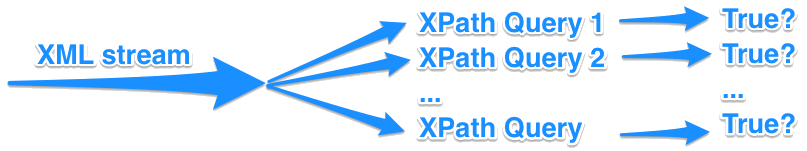
\includegraphics[width=\linewidth]{processing-problem.png}
    %\caption{<+caption text+>}
    %\label{fig:<+label+>}
  \end{figure}
\end{frame}

\begin{frame}{SAX}
  SAX is a type of parser implementing the following 5 methods
  \begin{itemize}
    \item[] \texttt{startDocument()}
    \item[] \quad\texttt{startElement(a)}
    \item[] \quad\quad\texttt{text(``3'')}
    \item[] \quad\texttt{endElement(a)}
    \item[] \texttt{endDocument()}
  \end{itemize}
  \dots simply translates to \mintinline{xml}{<a>c</a>}.
\end{frame}
\begin{frame}{The XML Filtering Problem}
  \begin{itemize}
    \item Definition:
      \begin{itemize}
        \item Given a set of XPath filters and a stream of XML documents, compute for each document $D$, the set of filters that match $D$.
      \end{itemize}
    \item The number of filters and predicates can be large (hundreds of thousands)
    \item Parallel / sequential query evaluation not scalable
  \end{itemize}
\end{frame}

\begin{frame}{Approach}
  \begin{itemize}
    \item Reduce the number of XPath predicate evaluations by
    \begin{itemize}
      \item Grouping common predicates 
      \item Evaluating (groups of) predicates once and reuse results
    \end{itemize}
  \end{itemize}
\end{frame}

\section{Method}
\begin{frame}{The XPush Machine}
  \begin{itemize}
    \item A modified \emph{deterministic\footnote{Lookup in O(1) time} pushdown automaton} (PDA)
    \item The PDA is constructed by alternating non-deterministic automatons (AFA)
    \item Each AFA is constructed by each XPath filter
  \end{itemize}
\end{frame}


\begin{frame}{AFA}
  \begin{minipage}{0.63\textwidth}
    \begin{itemize}
      \item P1=//a[b/text()=1 and .//a[@c>2]]
      \item P2=//a[@c>2 and b/text()=1]
    \end{itemize}
  \end{minipage}
  \begin{minipage}{0.35\textwidth}
  \begin{figure}
    \centering
    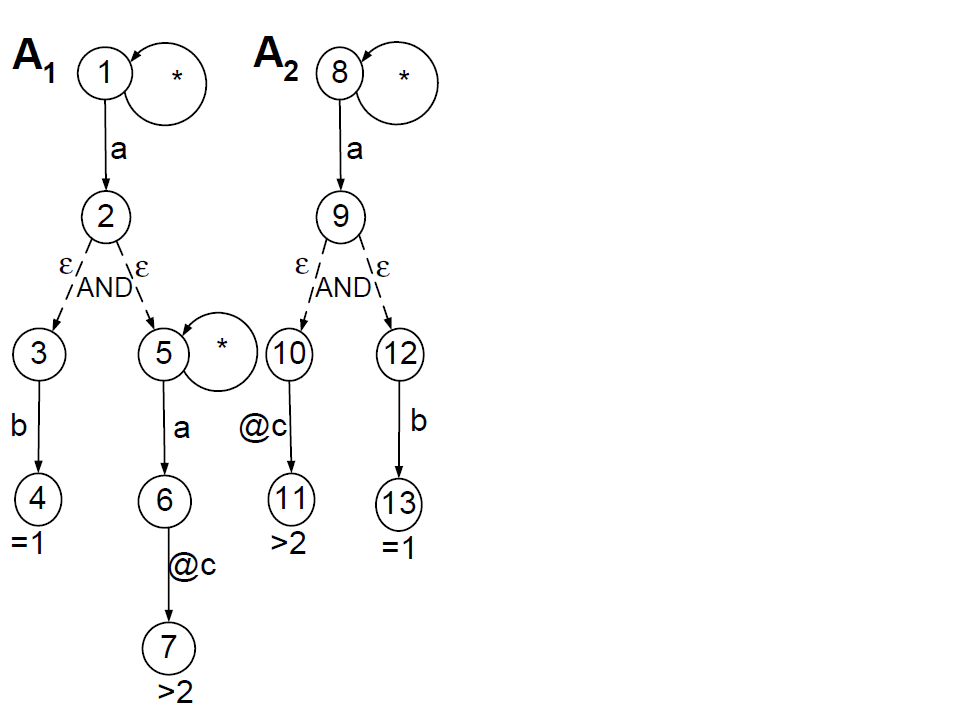
\includegraphics[width=\textwidth]{AFA.png}
  \end{figure}
\end{minipage}
\end{frame}

\begin{frame}{Constructing the XPush Machine}
  \begin{itemize}
    \item The XPush machine is computed lazily at runtime
    \begin{itemize}
      \item Computing all the states results in an exponential number of states
      \item Compute only those that are met at runtime
    \end{itemize}
    \item Each state in the XPush machine is a set of states in the AFAs and corresponds to a set of predicates in the XPath queries 
  \end{itemize}
\end{frame}

\section{Optimizations}
\begin{frame}{Methods of Optimization}
  \begin{itemize}
    \item Top-down pruning
    \item Order optimization
    \item Early notification optimization
    \item Training in the XPush machine
  \end{itemize}
\end{frame}

\begin{frame}{Top-down Pruning}
  \begin{itemize}
    \item Removes false positives
    \item For queries of the form e[c/text()=``c''], remove all predicates that does not appear under an \texttt{e} element\\ 
    \texttt{<e> \\
            \quad <c> ``c'' </c> \\
            \quad \dots \\
            \quad <c> ``c'' </c>\\ 
            </e>\\
            <a> \\
            \quad <c> ``c'' </c> \\
            </a>}
    \item Expensive to perform, but reduces number of states (reducing memory needed)
  \end{itemize}
\end{frame}

\begin{frame}{Order Optimization}
  \begin{itemize}
    \item If there is a order of elements defined in the DTD, we can faster find false filters
    \item If we have a query: \\\texttt{/person[name/text()="Smith" and age/text()="33" and phone/text()="5551234"]}
    \item And XML data: \\\texttt{<person><name>John</name><age>33</age> \dots}
    \item Then we can stop after the name predicate and not ``activate'' the age predicate
    \item Reduces average length of states and thus run time 
  \end{itemize}
\end{frame}

\begin{frame}{Early Notification Optimization}
  \begin{minipage}{0.63\textwidth}
  \begin{itemize}
    \item In early notification, the evaluation of a AFA in the XPush machine is stopped early once the first branching state has matched some node in the XML document
    \item Requires top-down pruning to ensure correctness
    \item Generated more states but reduces average length of states
  \end{itemize}
  \end{minipage}\quad
  \begin{minipage}{0.3\textwidth}
    \begin{figure}
      \centering
      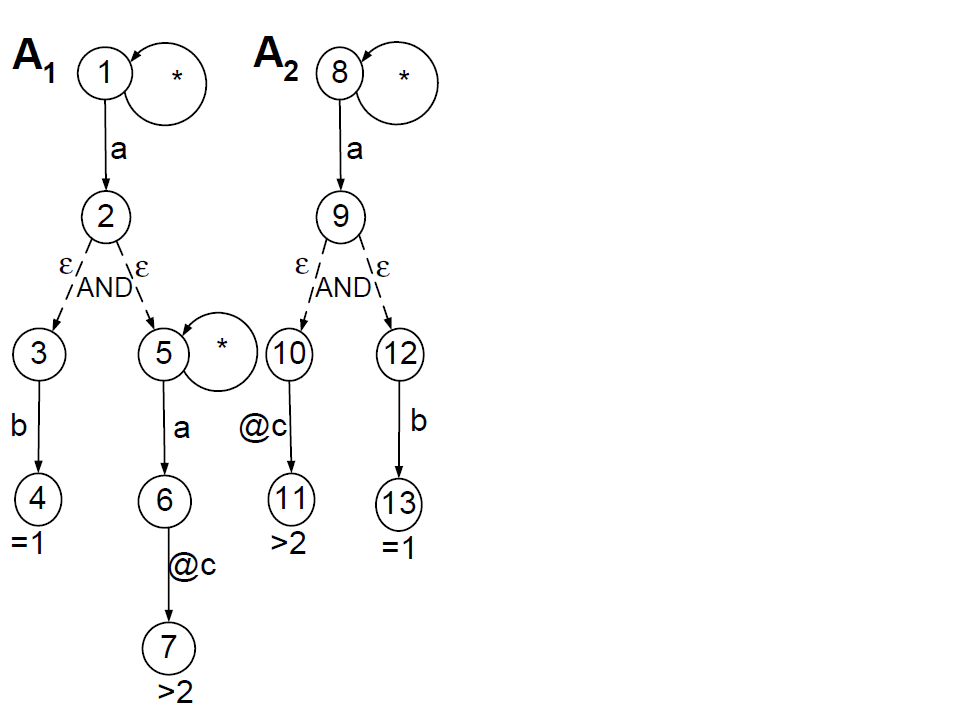
\includegraphics[width=\textwidth]{AFA.png}
    \end{figure}
  \end{minipage}

\end{frame}

\begin{frame}{Training in the XPush Machine}
  \begin{itemize}
    \item Generate training data from workload queries
    \begin{itemize}
      \item If we have \texttt{*} or \texttt{//} we can use the DTD
    \end{itemize}
    \item The DTD is also used to generate elements in the right order
    \item Precompute states based on the training data
    \item Can do lookup instead of runtime evaluation 
    \item Increases number of states but reduces average length of states
  \end{itemize}
\end{frame}

\section{Evaluation}
\begin{frame}{Number of States}
  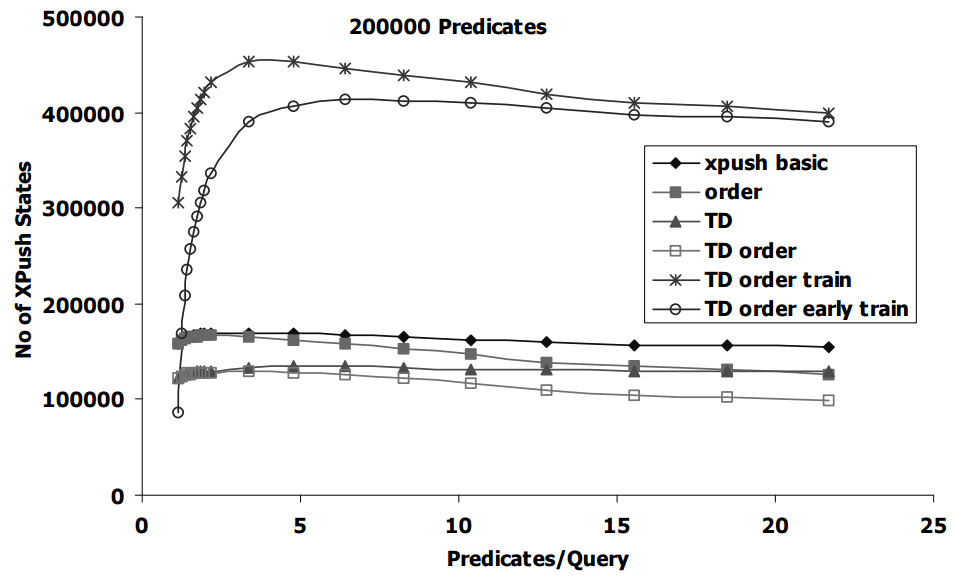
\includegraphics[width=\textwidth]{states}
\end{frame}

\begin{frame}{Average Length of States}
  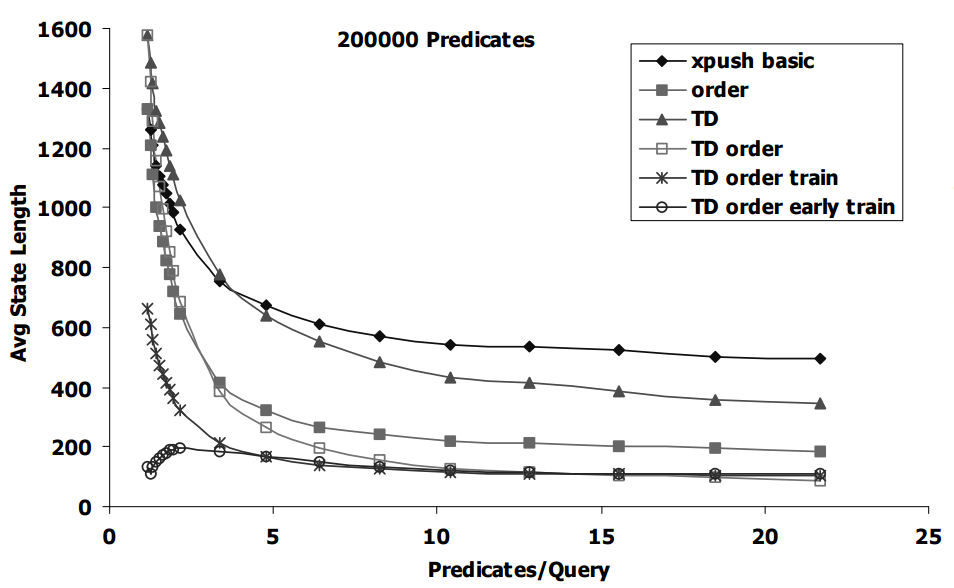
\includegraphics[width=\textwidth]{avglen}
\end{frame}

\begin{frame}{Filter Evaluation Time}
  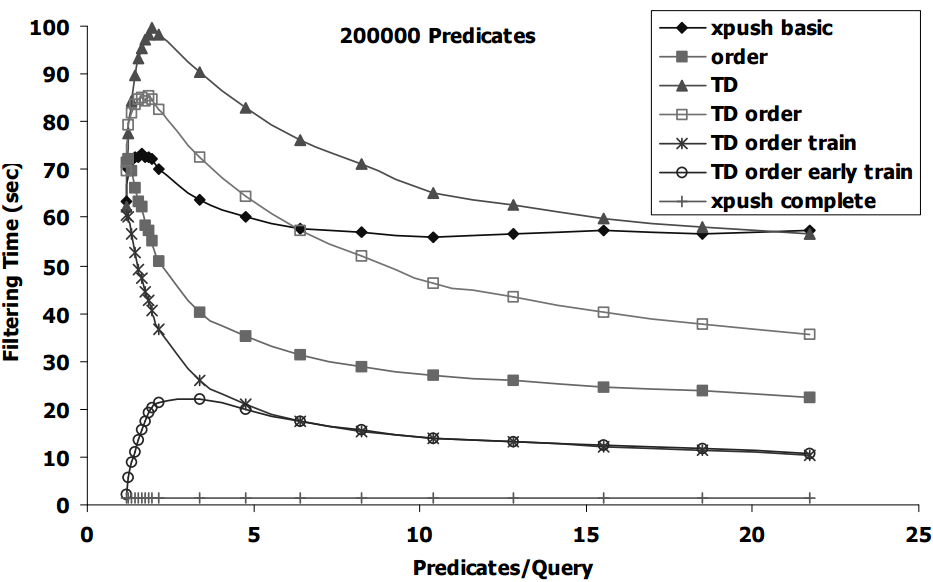
\includegraphics[width=\textwidth]{filtertime}
\end{frame}

\section{Limitations}
\begin{frame}{Limitations}
  \begin{itemize}
    \item Supports only a subset of XPath (e.g. no equal on ID)
    \item Can only stream a single document at a time
    \item Creation of states and AFAs is expensive
    \begin{itemize}
      \item If all the predicate are unique, falls back to normal execution + creating of AFAs
      \item Results in slow execution than not using this approach
    \end{itemize}
    \item The queries cannot be evaluated in parallel
    \item Updates to the XPath queries requires recomputing the XPush Machine from scratch
  \end{itemize}
\end{frame}

\section{Conclusion}
\begin{frame}{Conclusion}
  \begin{itemize}
    \item XPush machine is a modified PDA that processes each SAX event in $\mathcal{O}(1)$ time independent of the query workload
    \item The XPush machine needs to be lazily computed in most applications
    \item With their setup it ran almost twice as fast as the Apache parser (in 2003)
  \end{itemize}
\end{frame}
\end{document}
